	\documentclass[]{report}
\usepackage{tikz}
\newcommand{\inputtikz}[2]{%  
	\scalebox{#1}{\input{#2}}  
}
\usepackage[french]{babel}
\usepackage[utf8x]{inputenc}
\usepackage{amsmath}
\usepackage{graphicx}
%\usepackage[colorinlistoftodos]{todonotestfa}
\usepackage{listings}
\usepackage{color}
\usepackage{amsmath}
\usepackage{amsfonts}
\usepackage{mathtools}
\usepackage{graphicx}
\usepackage{caption}
\definecolor{dkgreen}{rgb}{0,0.6,0}
\definecolor{gray}{rgb}{0.5,0.5,0.5}
\definecolor{mauve}{rgb}{0.58,0,0.82}
%opening

\lstset
{frame=tb,
	language=R,
	aboveskip=3mm,
	belowskip=3mm,
	showstringspaces=false,
	framexleftmargin=5mm,
	columns= fixed,
	numbers = left,
	basicstyle={\small\ttfamily},	
	numberstyle=\tiny\color{gray},
	keywordstyle=\color{blue},
	commentstyle=\color{dkgreen},
	stringstyle=\color{mauve},
	breaklines=true,
	breakatwhitespace=true,
	tabsize=3
}

\begin{document}
	
\begin{titlepage}
	
	\newcommand{\HRule}{\rule{\linewidth}{0.5mm}} 
	
	\center 
	
	\textsc{\LARGE Université de Technologie de Compiegne}\\[1.5cm]
	\textsc{\Large SY09}\\[0.5cm] 
	\textsc{\large Data Mining}\\[0.5cm]
		
	\HRule \\[0.4cm]
	{ \huge \bfseries Premier Rendu}\\[0.4cm] 
	\HRule \\[1.5cm]
		
	\begin{minipage}{0.4\textwidth}
		\begin{flushleft} \large
			Oumaima \textsc{Talouka} 
		\end{flushleft}
	\end{minipage}
	~
	\begin{minipage}{0.4\textwidth}
		\begin{flushright} \large
			Zineb \textsc{SLAM} 
		\end{flushright}
	\end{minipage}\\[2cm]

	{\large \today}\\[2cm] 

	
\includegraphics[width=40mm]{Figures/utc.jpg}\\ % 

	\vfill
	
\end{titlepage}



\begin{abstract}
Dans ce rapport du TP1 de l'UV SY09 nous allons expliquer notre démarches dans l'analyse des données en expliquant les résultats obtenus. Ce TP est compose de 2 parties. La première partie a pour objectif de se familiariser avec les méthodes de traitement et de visualisation de données sur R. La deuxième partie traite de l'Analyse en composantes principales (ACP). Nous allons travailler avec 3 dataset notes de SY02, Crabs et Pima qu'on va d'abord analyser et décrire avant d'y réaliser l'ACP en seconde partie. Pour les graphes obtenus nous avons utilises la librairie ggplot2 qui offre un grand nombre de fonctionnalité Le code R sera fourni en annexe.

\end{abstract}

\tableofcontents

\chapter{ Statistique descriptive}

\section{Notes SY02}
Le dataset \textit{"sy02-p2016"} représente les notes des étudiants de l'UTC en SY02 ( statistiques) durant le printemps 2016. Nos données comptent \textit{N= 296} individus (étudiants) er \textit{p= 11} variables.  \textbf{Enlever les etudiants desinscrits}

 \subsection{Description des variables}

\begin{center}
	\begin{tabular}{c c }
		\textbf{Variables Quantitatives} & note.median, note.final, note.totale \\ 
		 \textbf{Variables Qualitatives Nominales} & nom, specialite, status, dernier.diplome.obtenu, correcteur.median, correcteur.final\\
		  \textbf{Variables Qualitatives Ordinales}  & niveau, resultat  \\
	\end{tabular}
	\captionof{table}{Categorie de Variables}
\end{center} 

\begin{itemize}
	\item \textbf{Nom:} chaine de caractère des identifiants de chaque étudiant
	\item \textbf{Spécialité:} la branche de l'etudiant: GB, GM, GSM, GP, GI
	\item \textbf{Niveau}: Semestre de l'etudiant de 1 a 6
	\item \textbf{Statut}: Soit l'étudiant est de l'UTC ou en semestre d'échange
	\item \textbf{dernier.diplome.obtenu:}
	BAC, DUT, CPGE, ETRANGER SUPERIEUR, LICENCE, OTHER, NA
	\item \textbf{Note Médian:} note de l'examen Médian
	\item \textbf{Correcteur Médian:} ID du correcteur du médian de 1 a 8. 
	\item \textbf{Note.final:} Note de l l'examen final
	\item \textbf{Note.totale:} Note totale obtenue a partir de la note du médian et la note du final
	\item \textbf{Correcteur.final}: D du correcteur du final de 1 a 8. 
	\item \textbf{Résultat}: Résultat obtenu de SY02 : A, B, C, D, E et F.
\end{itemize}

Pour les notes de médian et de final il y'a des notes non mentionnées (NA) par contre tous les etudiants ont un résultat final c'est pour cela on n'a pas enlevé les etudiants avec NA en médian ou/et en final.\\
Les variables importantes dans ce dataset sont les résultats des etudiants et comment ceux ci sont influences par d'autre variable, par exemple le niveau et la spécialité\\
Il est évident qu'il existe une relation linéaire entre ces 3 variables: note.median, note.final et note.totale vu que la note totale est exprimée par une relation linéaire entre la note.median et la note.final (par exemple $note.totale = 40\% * note.median + 40\% * note.final + cste$). La variable note.totale et la variable resultat sont des variables fortement corrélés En effet le résultat est une "traduction"  de la note totale. On pourrait éventuellement se demander sur la relation entre les notes et le niveau, la spécialité, le diplôme ainsi que le correcteur. C'est ce qu'on va essayer d'analyser dans ce qui suit. 

 \subsection{Analyse descriptive des données}

\subsubsection{Lien entre les variables}
	\begin{center}
	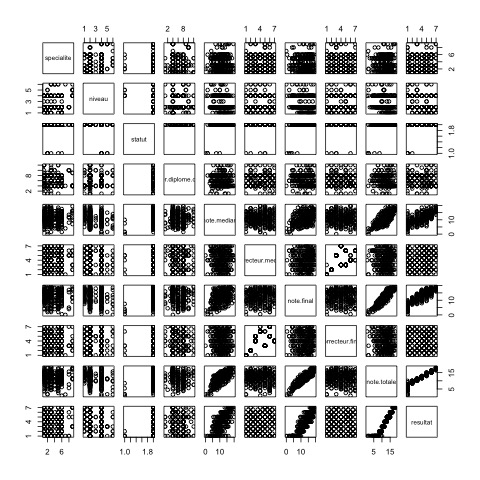
\includegraphics[width=50mm]{Figures/Notes/multiplot.jpg}
	\captionof{figure}{Plot general}
	\label{fig:multiplot_notes}
\end{center}

\subsubsection{Performance et homogénéité}
La figure ci-dessous représente trois diagrammes a boites des notes de médian, final et le résultat de l'UV SY02.
	\begin{center}
			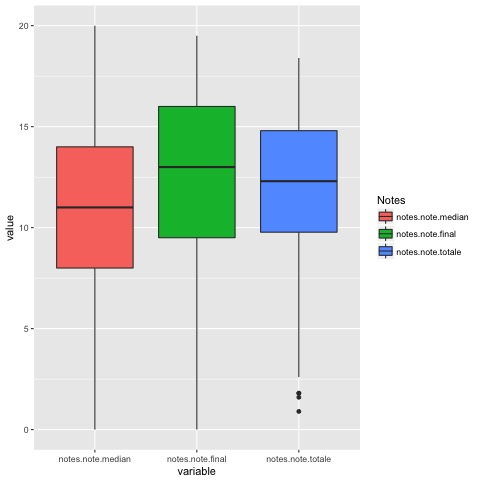
\includegraphics[width=50mm]{Figures/Notes/boxplot_exam.jpg}
			\captionof{figure}{Boxplot des Notes de Median, Final et Totale}
		    \label{fig:Boxplot_notes}
	\end{center}

On remarque que par passage du médian au final les notes ont augmente. En effet ceci est aussi témoigné par le tableau ci-dessous:

\begin{center}
	\begin{tabular}{c c c c c }
		\textbf{Notes} & \textbf{1er Quartl} & \textbf{Medianne}   & \textbf{Moyenne} & \textbf{3em Quartl} \\
		Median  & 8.0 			& 11.0		 & 10.92      & 14.0\\
		Final      & 9.50 		  & 13.0 	   & 12.38	    & 16.0\\
		Totale   & 9.775        & 12.3       &  11.845    & 14.8\\
	\end{tabular}
	\captionof{table}{Notes}
\end{center} 

Il est tout a fait logique que le digramme de résultats se situe entre les 2 puisque que c'est la moyenne \textbf{pondérée??} des 2 notes.
 
	
\subsubsection{Lien entre la réussite, la formation, la branche et le niveau}

	\begin{center}
	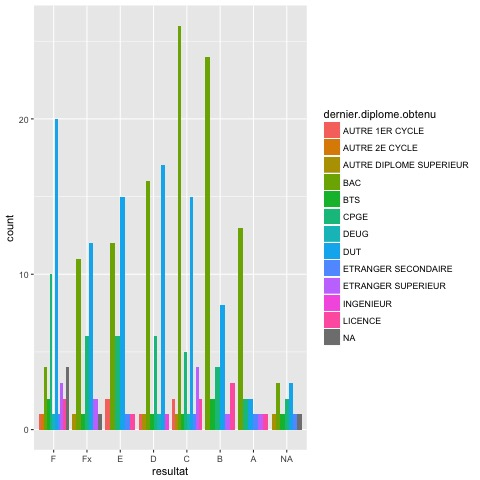
\includegraphics[width=50mm]{Figures/Notes/diplome_resultat.jpg}
	\captionof{figure}{Diagramme a baton de lien entre la formation et le resultat}
	\label{fig:formation_resultat}
	\end{center}



	\begin{center}
	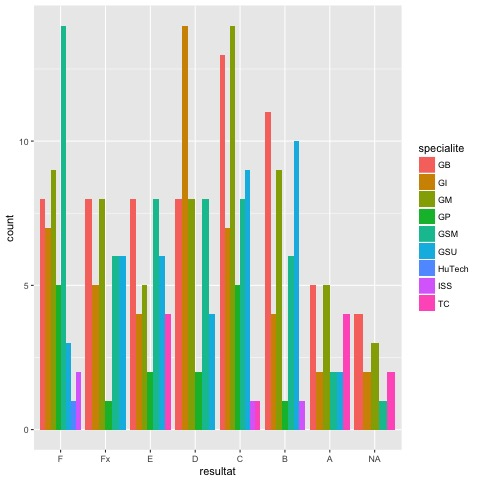
\includegraphics[width=50mm]{Figures/Notes/specialite_resultat.jpg}
	\captionof{figure}{Diagramme a baton de lien entre la branche et le resultat}
	\label{fig:specialite_resultat}
	\end{center}


		\begin{center}
		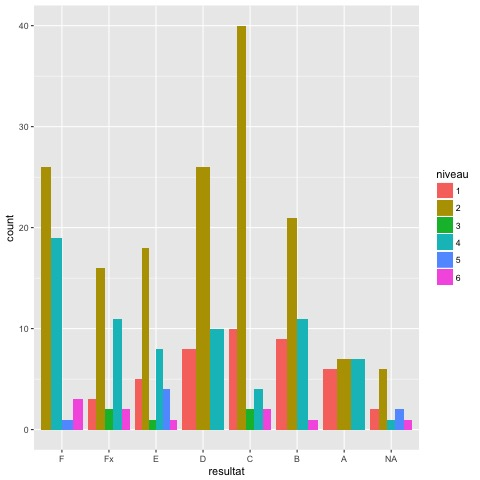
\includegraphics[width=50mm]{Figures/Notes/niveau_resultat.jpg}
		\captionof{figure}{Diagramme a baton de lien entre le niveau et le resultat}
		\label{fig:niveau_resultat}
		\end{center}

\subsubsection{Influence du correcteur sur la note}

	\begin{center}
	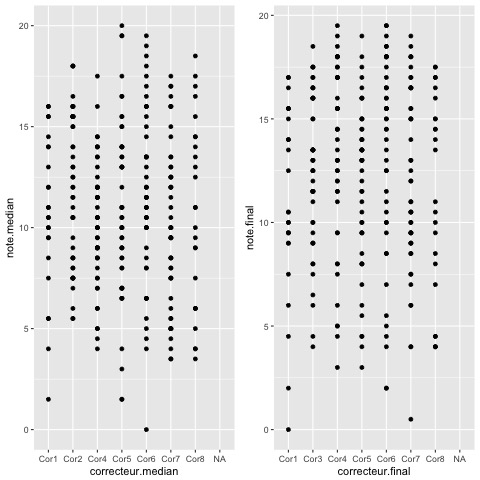
\includegraphics[width=70mm]{Figures/Notes/correcteur.jpg}
	\captionof{figure}{Scatterplot des notes en fonction des correcteurs}
	\label{fig:scatter_correcteur_median}
\end{center}

\section{Conclusion}

\section{Crabs}

\section{Pima}

\chapter{Analyse Composantes Principales}
\end{document}
